\subsection{USB-B}
\label{subsec:USB-B}

Auf der Leiterplatte des PartyMixer's gibt es zwei Komponenten, welche programmiert werden müssen. Der Mikrocontroller und das WiFi-Modul. Um diese zu programmieren braucht es eine entsprechende Schnittstelle, welche mit einer USB-B-Schnittstelle realisiert wird.

Die USB-B-Schnittstelle benötigt nur zwei Kommunikationsleitungen (D+ und D-), die zu programmierenden Geräte benötigen mehr Anschlüsse um in einen Programmiermodus zu kommen oder mit den Geräten zu Kommunizieren. Deswegen benötigt es einen USB-UART-Converter. Hier wurde einerseits auf das Flash-Interface von Arduino zurückgegriffen, um die Schaltung für den Mikrocontroller zu planen \cite{arduino_cc_arduino_2017} und auf das Flash-Interface des ESP32, um die Schaltung für den ESP32 zu planen \cite{espressif_systems_esp32_2016}. In der Tabelle \ref{tab:USB_uC} wird dargestellt, welche Leitungen für das jeweilige Flash-Interface benötigt werden. Die USB-B-seitige Schnittstelle wird an den Computer angeschlossen und muss nicht häher betrachtet werden.

\begin{table}[h!]
\center
\begin{tabular}{|c|lcl|c|}
\hline
\textbf{Mikrocontroller} & & & & \textbf{USB-Flash-Device} \\ \hline
RX & <== & direkt & === & TX  \\
TX & === & direkt & ==> & RX  \\
Reset & <== & Kondensator & === & DTR \\
\hline
\end{tabular}
\label{tab:USB_uC}
\caption{Verbindung zwischen USB und Mikrocontroller.}
\end{table}

\begin{table}[h!]
\center
\begin{tabular}{|c|lcl|c|}
\hline
\textbf{ESP} & & & & \textbf{USB-Flash-Device} \\ \hline
RX & <== & direkt & === & TX  \\
TX & === & direkt & ==> & RX  \\
EN & <== & über Transistor & === & RTS \\
IO\_0 & <== & über Transistor & === & DTR \\
IO\_13 & <== & über Widerstand & === & RTS \\
IO\_15 & <== & über Widerstand & === & CTS \\
\hline
\end{tabular}
\label{tab:USB_ESP}
\caption{Verbindung zwischen USB und ESP.}
\end{table}

Um in den automatischen Programmiermodus zu kommen, muss folgender Handshake zwischen den Geräten stattfinden:

\paragraph{ATMega2560 Handshake}\mbox{}

GPIO\_0:

Low/GND = ROM serial bootloader for esptool.py

High/VCC = Normal execution mode

Has internal Pullup resistor

Button: ''Flash'' oder ''BOOT'' on development boards. Pulls GPIO\_ 0 low when pressed.

GPIO\_ 2:

must be either left unconnected/floating, or driven low, in order to enter the serial bootloader

in normal boot mode (GPIO\_ 0 high), GPIO\_ 2 is ignored

GPIO\_ 12 (MTDI)

if driven high, flash voltage is 1.8V, not default 3.3V.

could cause the flash to brownout.

GPIO\_ 15 (MTDO)

If driven low, silences boot messages printed by the ROM bootloader.

Has internal Pull-up ==> High = normal output

\paragraph{ESP32 Handshake}\mbox{}

In der folgenden Tabelle \ref{tab:Einfluss_Pins_auf_Boot_Modus} wird der Einfluss der Pins auf den Boot-Modus aufgezeigt.

\begin{table}[h!]
\center
\begin{tabular}{|l|c|c|c|}
\hline
\multicolumn{4}{|c|}{Boot-Mode Konfiguration}\\
\hline
Pin & Default & Boot & Download \\
\hline
IO0 & 1 & 1 & 0 \\
\hline
U0TXD & 1 & 1 & X \\
\hline
IO2 & 0 & X & 0 \\
\hline
IO4 & 0 & X & X \\
\hline
IO15 & 1 & X & X \\
\hline
IO5 & 1 & 1 & X \\
\hline
\end{tabular}
\caption{Wenn U0TXD, IO2, IO5 floating sind, bestimmt IO0 den Boot-Modus.}
\label{tab:Einfluss_Pins_auf_Boot_Modus}
\end{table}

Mit dieser Tabelle

%Auch hier wurde vom Arduino Uno-Board abgekpufert und der selbe Chip verwendet, um die USB-Signale in UART-Signale zu konvertieren. Das vorkommende Bauteil ist der CP2102N. Da dieser Chip ein TQFP-28-Gehause hat, könnte es auch schwierigkeiten geben beim Löten. Deswegen wird auch ein Breakout-Board (BOB) mitgeplant, damit es eine Ausweichmöglickeit gibt falls die Bauteile zu klein sind.

%\begin{figure}[!h]
%\center
%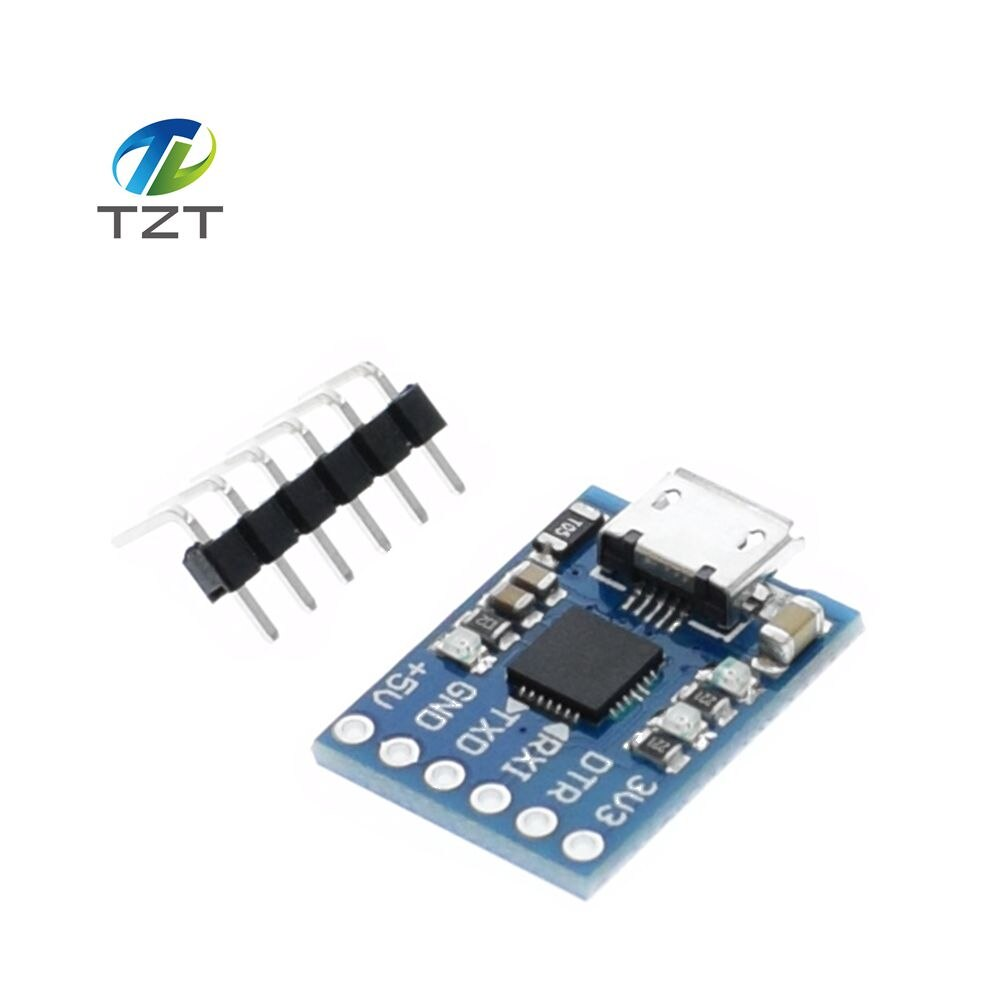
\includegraphics[width = 0.5\textwidth]{graphics/Produktbild_USB_UART_uC}
%\caption{CP2102N-BOB für uC.}
%\label{fig:Produktbild_USB_UART_uC}
%\end{figure}
%
%\begin{figure}[!h]
%\center
%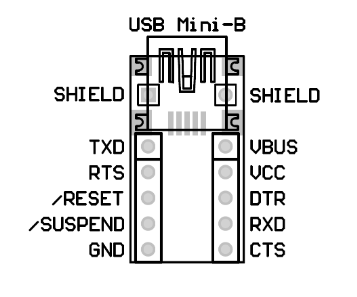
\includegraphics[width = 0.5\textwidth]{graphics/Produktbild_USB_UART_ESP}
%\caption{CP2102N-BOB für ESP.}
%\label{fig:Produktbild_USB_UART_ESP}
%\end{figure}